%
% Copyright (c) 2020 Antonio Coín Castro
%
% This work is licensed under a
% Creative Commons Attribution-ShareAlike 4.0 International License.
%
% You should have received a copy of the license along with this
% work. If not, see <http://creativecommons.org/licenses/by-sa/4.0/>.

We begin this work by presenting the fundamentals of \textit{fuzzy theory}. This theory was developed by computer scientist and mathematician Lofti A. Zadeh around 1965 (see \cite{zadeh1965fuzzy}). He felt the need to introduce a concept that would enable the treatment of systems in an imprecise manner, due to lack of information or simply because of some inherent ambiguity. At the same time, he wanted this notion to be mathematically coherent and tractable, and to have a strong theoretical base from which to expand to practical applications.

With these ideas in mind he established the concepts of \textit{fuzzy sets} and \textit{fuzzy reasoning}, providing a robust foundation for developing various methods to deal with uncertainty and impreciseness. These methods are widely used nowadays in the construction of control systems and the modelling of situations which involve a certain degree of vagueness, uncertainty or ambivalence.

The main references for this chapter are \cite{chen2000introduction} and \cite{jang1997neuro}, from which we extract some basic definitions and a handful of results to illustrate the extent of this theory.

\section{Fuzzy set theory}

\subsection{Basic concepts}

Let $X$ be a space of objects, known as the \textit{universe of discourse}. Where necessary in our discussion, we may assume that $X = \mathbb{R}$. We begin with the most basic definition, which sets the ground rules for all the theory that will be developed.

\begin{definition}[Fuzzy set] A fuzzy set $A$ in $X$ is the set of ordered pairs
\[
A = \{ (x, \mu_A(x)) \ | \ x \in X \},
\]
where $\mu_A(x)$ is the \textit{membership function} (\acrshort{mf}) for the fuzzy set $A$. It maps each element of $X$ to a membership grade in $[0,1]$.
\end{definition}

Thus, a fuzzy set is uniquely specified by its membership function, which measures the degree to which every element of the universe belongs to this particular set. Because of this, an abuse of notation will sometimes be allowed when using only a membership function to denote the underlying fuzzy set. An alternative way of denoting a fuzzy set $A$ is as follows:
\begin{align*}
& A = \sum_{x_i \in X} \mu_A(x_i) \slash x_i, \ \ \text{if $X$ is discrete,} \\
& A = \int_X \mu_A(x) \slash x, \ \ \text{if $X$ is a continuous space.}
\end{align*}

\begin{remark}
	If $\mu_A(x)$ is restricted to $\{0,1\}$, then $A$ becomes a set in the classical sense (which will be referred to as a \textit{crisp set}). We note that the fundamental distinction between a crisp set and a fuzzy set is that the latter introduces a measure of uncertainty to model the notion of an element belonging to a certain group, which can be useful in real-life scenarios.
\end{remark}

We now present a couple of concepts that help summarize the characteristics of our newly defined fuzzy sets.

\begin{definition}[Support] The support of a fuzzy set $A$ is the set of all points $x \in X$ such that $\mu_A(x) > 0$.
\end{definition}

\begin{definition}[Core] The core of a fuzzy set $A$ is the set of all points $x \in X$ such that $\mu_A(x) = 1$.
\end{definition}

\begin{definition}[Normality] A fuzzy set $A$ is \textit{normal} if its core is nonempty, that is, if there exists some $x \in X$ such that $\mu_A(x) = 1$.
\end{definition}

\begin{definition}[Crossover points] A crossover point of a fuzzy set is a point $x \in X$ for which $\mu_A(x) = 0.5$:
\[
\operatorname{crossover}(A) = \{ x \ | \ \mu_A(x) = 0.5 \}.
\]

\end{definition}

\begin{definition}[Fuzzy singleton] A fuzzy set whose support is a single point in $X$ with $\mu_A(x) = 1$ is called a fuzzy singleton.

\end{definition}

\begin{definition}[$\alpha$-cut, strong $\alpha$-cut] The $\alpha$-cut or \textit{$\alpha$-level set} of a fuzzy set $A$ is defined for $\alpha \in [0,1]$ as follows:
\[
A_\alpha = \{ x \ | \ \mu_A(x) \ge \alpha \}.
\]
Similarly, the strong $\alpha$-cut, or \textit{strong $\alpha$-level set} $A'_\alpha$ is defined by replacing '$\ge$' with '$>$'.

\end{definition}

\begin{remark} With the notation for level sets, it is clear that $\operatorname{support}(A) = A'_0$ and $\operatorname{core}(A) = A_1$.

\end{remark}

The concept of level sets plays an important role in the theory of fuzzy sets, as they provide a way of characterizing these entities using only crisp sets. This behaviour is exemplified in the following theorem.

\begin{theorem}[Resolution principle] Every MF can be decomposed into a combination of its $\alpha$-level sets' MFs:
\[
\mu_A(x) = \sup_\alpha \, \min \left\{ \alpha, \mu_{A_\alpha}(x) \right\}.
\]
Remember that $A_\alpha$ is a crisp set and thus $\mu_{A_\alpha}$ is understood as its characteristic function, taking values in $\{0,1\}$.
\end{theorem}
\begin{proof}
  Let $x \lor y$ denote the operation $\max \{x,y\}$ and $x \land y$ denote $\min\{x,y\}$. Then it follows that for every $x\in X$,
  \begin{align*}
    \sup_\alpha \left\{ \alpha \land \mu_{A_\alpha}(x) \right\} &= \sup_{\alpha \in [0,\mu_A(x)]} \left\{ \alpha \land \mu_{A_\alpha}(x) \right\} \lor \sup_{\alpha \in [\mu_A(x), 1]} \left\{ \alpha \land \mu_{A_\alpha}(x) \right\}\\
    &= \sup_{\alpha \in [0,\mu_A(x)]} \left\{ \alpha \land 1 \right\} \lor \sup_{\alpha \in [\mu_A(x), 1]} \left\{ \alpha \land 0 \right\}\\
    &= \sup_{\alpha \in [0,\mu_A(x)]} \left\{ \alpha  \right\} \lor 0\\
    &= \mu_A(x).
  \end{align*}

\end{proof}

Lastly, we finish this section with yet another set of definitions, concerned mainly with the shape that fuzzy sets can adopt. These concepts will be useful later on when describing specific MFs.

\begin{definition}[Convexity] A fuzzy set $A$ is \textit{convex} if for any $x_1,x_2 \in X$ and any $\lambda \in [0,1]$, it holds that
\[
\mu_A(\lambda x_1 + (1-\lambda)x_2) \ge \min{\{ \mu_A(x_1), \mu_A(x_2)\}}.
\]
Alternatively, $A$ is convex if all its $\alpha$-level sets are convex (i.e. composed of a single line segment only).
\end{definition}

\begin{definition}[Fuzzy number] A fuzzy number is a fuzzy set in $\mathbb{R}$ that is both normal and convex.
\end{definition}

\begin{definition}[Symmetry] A fuzzy set $A$ is said to be \textit{symmetric} around a point $c \in X$ if it satisfies
\[
\mu_A(c + x) = \mu_A(c - x), \quad \text{for all } x \in X.
\]

\end{definition}

\begin{definition}[Open left, open right, closed] A fuzzy set $A$ is said to be \textit{open left} if $\displaystyle \lim_{x \to -\infty} \mu_A(x) = 1$ and $\displaystyle\lim_{x \to \infty} \mu_A(x) = 0$; \textit{open right} if $\displaystyle\lim_{x \to -\infty} \mu_A(x) = 0$ and $\displaystyle\lim_{x \to \infty} \mu_A(x) = 1$; and \textit{closed} if $\displaystyle\lim_{x \to \pm \infty} \mu_A(x) = 0$.

\end{definition}

In most applications it makes sense to work with convex membership functions, since they are easy to visualize and interpret. An example visualization to help us differentiate between convex and nonconvex fuzzy sets can be seen in Figure \ref{fig:convex-fuzzy}.
\begin{figure}[h!]
\centering
\begin{subfigure}{.4\textwidth}
  \centering
  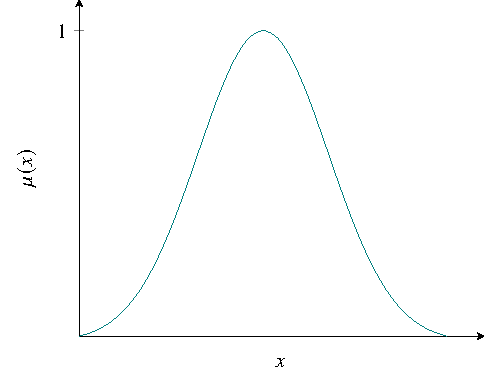
\includegraphics[width=.8\linewidth]{convex-fuzzy}
  \caption{Convex fuzzy set}
  \label{fig:sub-first}
\end{subfigure}
\begin{subfigure}{.4\textwidth}
  \centering
  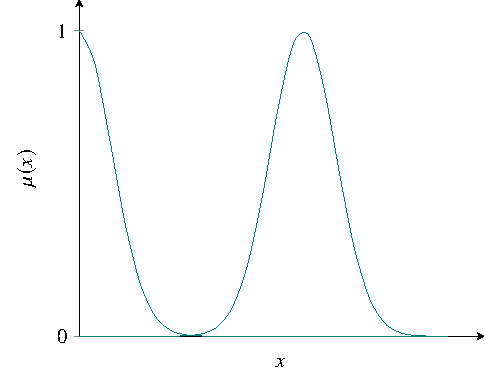
\includegraphics[width=.8\linewidth]{nonconvex-fuzzy}
  \caption{Nonconvex fuzzy set}
  \label{fig:sub-second}
\end{subfigure}
\caption{Representation of membership functions of convex and nonconvex fuzzy sets.}
\label{fig:convex-fuzzy}
\end{figure}


%--------------------------------------
%   Set-Theoretic Operations
%--------------------------------------

\subsection{Set-theoretic operations}

Most set-theoretic operations in the classical theory translate to fuzzy set theory in a natural way. We present a list of some of the most basic of these operations and their reinterpreted definitions in our setting, while introducing some of the notation that will be used in what follows.

\begin{definition}[Subset] If $A$ and $B$ are fuzzy sets, we say that $A$ is a subset of $B$, and we write $A \subseteq B$, if $\mu_A(x) \le \mu_B(x)$ for all $x \in X$.
\end{definition}

\begin{definition}[Union] The union of two fuzzy sets $A$ and $B$ is a fuzzy set $C = A \cup B$, whose MF is $\mu_C(x) = \max \, \{\mu_A(x), \mu_B(x) \} = \mu_A(x) \lmax \mu_B(x)$.
Alternatively, we can say that $C$ is the ``smallest'' fuzzy set that contains both $A$ and $B$.
\end{definition}

\begin{definition}[Intersection]
The intersection of two fuzzy sets $A$ and $B$ is a fuzzy set $C = A \cap B$, whose MF is $\mu_C(x) = \min \, \{\mu_A(x), \mu_B(x) \} = \mu_A(x) \lmin \mu_B(x)$.
As in the case of the union, $C$ can be viewed as the ``largest'' fuzzy set contained in both $A$ and $B$.
\end{definition}

\begin{definition}[Complement] The complement of a fuzzy set $A$, denoted by $\bar A$, is another fuzzy set defined by $\mu_{\bar A}(x) = 1- \mu_A(x)$.

\end{definition}

\begin{definition}[Cartesian product and co-product]
Let $A$ and $B$ be fuzzy sets in $X$ and $Y$, respectively. The \textit{Cartesian product} $A \times B$ is a fuzzy set in $X \times Y$ given by
\[
\mu_{A \times B}(x,y) = \mu_A(x) \lmin \mu_B(y).
\]
Similarly, the \textit{Cartesian co-product} $A+B$ is a fuzzy set in $X \times Y$ which has the membership function
\[
\mu_{A + B}(x,y) = \mu_A(x) \lmax \mu_B(y).
\]

\end{definition}

As it turns out, there are various ways of defining these basic operations in a fuzzy context, so we will refer to the operators used above as the \textit{classical} or \textit{standard fuzzy operators}. Other operators are discussed briefly in Subsection \ref{ssec:tnorm}. The choice of a specific fuzzy operator will depend on the specific problem we try to model, since different operators will most likely yield different outcomes and conclusions.

As with any new mathematical structure, one of the first steps after studyng its basic properties is to study which operations preserve this structure, and how to generate new entities from existing ones. Regardless of the concrete operators employed, the operations just described provide us with the ability of generating new fuzzy sets from existing ones, while maintaining a reasonable interpretation of what they represent. Some of them will even preserve interesting properties of fuzzy sets, as seen in next result, whose proof can be derived by merely writing down the definitions of the concepts involved.

\begin{prop} An arbitrary intersection of convex fuzzy sets is a convex fuzzy set.
\end{prop}

Continuing along the same lines, we arrive at an important theorem regarding the creation of new fuzzy sets, stated by Zadeh himself. In short, it says that we can generate a fuzzy set that represents any structure, concept or relation that can be described with a (classical) mapping. A detailed introduction to this result and some insight as to its usefulness is given by E. Kerre in \cite{kerre2011tribute}.

\begin{theorem}[Extension principle] Let $f$ be a mapping from an $n$-dimensional product space $X_1 \times \dots \times X_n$ to a one-dimensional universe $Y$, and suppose $A_1, \dots, A_n$ are $n$ fuzzy sets in $X_1, \dots, X_n$, respectively. Then $f$ induces a fuzzy set $B$ in $Y$ defined by
\[
\mu_B(y) = \left\{ \begin{array}{cc}
	\sup\limits_{(x_1, \dots, x_n) = f^{-1}(y)} \, \min\limits_i \, \{ \mu_{A_i}(x_i) \}, & \text{if } f^{-1}(y) \ne \emptyset, \\
	0, & \text{if } f^{-1}(y) = \emptyset.
\end{array}\right.
\]

\end{theorem}

\begin{corollary} Let $f:X \to Y$ be a one-to-one mapping between one-dimensional spaces, and let $\mu_A$ represent a fuzzy set in $X$. Then, a fuzzy set $\tilde{f}(A)$ is induced in $Y$, given by
\[
\tilde{f}(A) = \int_X \mu_A(x) \slash f(x).
\]

\end{corollary}

\begin{example} Let $+:\R^2 \to \R$ represent the usual addition operation. Using the extension principle we can define the sum of two fuzzy sets $A$ and $B$ in $\R$ as a new fuzzy set $A+B$ with membership function given by
\[
\mu_{A+B}(z) = \sup \, \{\mu_A(x) \land \mu_B(y) \ | \ z = x + y \}, \quad \forall z \in \R.
\]

\end{example}

To conclude this brief exposition of operations between fuzzy sets, we now consider the general setting in which we have a multidimensional universe (i.e, a product space). In this case, it can be useful to think of fuzzy sets as a \textit{relation} among tuples of elements, each of which has a membership grade to the implied fuzzy set.

\begin{definition}[Fuzzy relation] Let $X$ and $Y$ be two universes of discourse. Then the fuzzy set
\[
\mathcal R = \{ ((x,y), \, \mu_\mathcal R (x,y) ) \ | \ (x,y) \in X \times Y \}
\]
represents a \textit{binary fuzzy relation} in $X \times Y$. A generalization to $n$-ary relations is straightforward.

\end{definition}

If $X$ and $Y$ are both discrete, we can express a fuzzy relation as a relation matrix $\mathcal R = (r_{ij})$, where $r_{ij}$ is the membership grade between the $ith$ element of $X$ and the $jth$ element of $Y$. As with fuzzy sets, we can operate with relations to produce new fuzzy sets, again using the classical operators previously described.

\begin{definition}[Max-min composition] \label{def:maxmin} Let $\mathcal{R}_1$ and $\mathcal{R}_2$ be two fuzzy relations defined on $X \times Y$ and $Y \times Z$, respectively. The max-min composition of $\mathcal R_1$ and $\mathcal R_2$ is a fuzzy set $\mathcal R_1 \circ \mathcal R_2$ in $X \times Z$ defined by
\[
\mu_{\mathcal R_1 \circ \mathcal R_2}(x,z) = \max_{y} \, \{ \mu_{\mathcal R_1}(x,y) \land \mu_{\mathcal R_2}(y,z) \}.
\]

\end{definition}

\begin{remark} If $\mathcal R_1$ and $\mathcal R_2$ are relation matrices, the calculation of $\mathcal R_1 \circ \mathcal R_2$ is almost the same as matrix multiplication, except that $\times$ and $+$ are replaced by $\land$ and $\lor$, respectively.

\end{remark}

\begin{prop} Let $\mathcal R, \mathcal S$ and $\mathcal T$ be binary relations on $X \times Y$, $Y \times Z$ and $Z \times W$, respectively, and let $\circ$ denote the max-min composition. Then, the following properties hold:

\begin{enumerate}
\item (Associativity) \ $\mathcal R \circ (\mathcal S \circ \mathcal T) = (\mathcal R \circ \mathcal S) \circ \mathcal T$;
\item (Distributivity  over union) \ $\mathcal R \circ (\mathcal S \cup \mathcal T) = (\mathcal R \circ \mathcal S) \cup (\mathcal R \circ \mathcal T)$;
\item (Weak distributivity over intersection) \ $\mathcal R \circ (\mathcal S \cap \mathcal T) \subseteq (\mathcal R \circ \mathcal S) \cap (\mathcal R \circ \mathcal T)$;
\item (Monotonicity) \ $\mathcal S \subseteq \mathcal T \implies \mathcal R \circ \mathcal S \subseteq \mathcal R \circ \mathcal T$.
\end{enumerate}

\end{prop}

\begin{proof}
  All four properties are easy to verify and follow directly from the well-known properties of the operators $\land$ and $\lor$.
\end{proof}

As one could expect, there are many possible definitions for a composition operator. For instance, another type of composition used in the literature (see \cite{markovsii2004solution, loetamonphong2001optimization}) is the \textit{max-product composition}.

\begin{definition}[Max-product composition] Assuming the same notation as above, the max-product composition is defined as follows:
\[
\mu_{\mathcal R_1 \circ \mathcal R_2}(x,z) = \max_{y} \, \{ \mu_{\mathcal R_1}(x,y) \mu_{\mathcal R_2}(y,z) \}.
\]

\end{definition}

%--------------------------------------
%   One-dimensional MFs
%--------------------------------------

\subsection{Parametrized one-dimensional MFs}

In this section, we describe the classes of parametrized functions commonly used to define one-dimensional fuzzy sets.

\begin{definition}[Triangular MF] Three parameters determine the $x$-coordinates of the three corners of a triangle:
\[
\operatorname{triangle}(x;a,b,c) = \max \left\{ \min \left\{ \frac{x-a}{b-a},\frac{c-x}{c-b}  \right\}, 0\right\}.
\]

\end{definition}

\begin{definition}[Trapezoidal MF] Four parameters determine the $x$-coordinates of the four corners of a trapezoid:
\[
\operatorname{trapezoid}(x;a,b,c,d) = \max \left\{ \min \left\{ \frac{x-a}{b-a},1, \frac{d-x}{d-c}  \right\}, 0\right\}.
\]

\end{definition}

\begin{definition}[Gaussian MF] It is determined by its center ($c$) and its width ($\sigma$) as follows:
\[
\operatorname{gaussian}(x;c,\sigma) = \exp \left(-\frac{1}{2}\left( \frac{x-c}{\sigma} \right)^2\right).
\]

\end{definition}

\begin{definition}[Generalized bell MF] It is specified by three parameters:
\[
\operatorname{bell}(x;a,b,c) = \frac{1}{1 + \left| \frac{x-c}{a}\right|^{2b}},
\]
where $b$ is usually positive.

\end{definition}

\begin{definition}[Sigmoidal MF] A sigmoidal MF is defined by
\[
\operatorname{sig}(x;a,c) = \frac{1}{1 + e^{-a(x-c)}},
\]
where $a$ controls the slope at the crossover point $x=c$.

\end{definition}

\begin{remark} Depending on the sign of the parameter $a$, a sigmoidal MF is inherently open right or left, and thus asymmetric. Closed and asymmetric MFs can be synthesized using either the absolute difference or the product of two sigmoidal functions.

\end{remark}

Triangular and trapezoidal membership functions are used because of their simplicity, both computational and interpretative. Nonetheless, they are composed of line segments and thus are not differentiable. This is where smooth MFs such as the Gaussian MF come into play, proving their usefulness in certain scenarios such as neuro-fuzzy systems. Some of these membership functions are shown in Figure \ref{fig:mfs}.


\begin{figure}[h!]
    \centering
    \begin{subfigure}[b]{0.4\textwidth}
        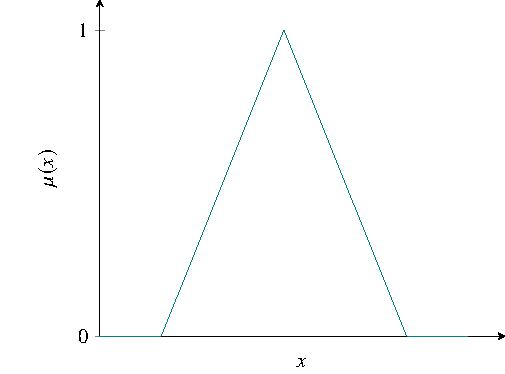
\includegraphics[width=\textwidth]{mf-triangle}
        \caption{Traingular MF}
    \end{subfigure}
    \begin{subfigure}[b]{0.4\textwidth}
        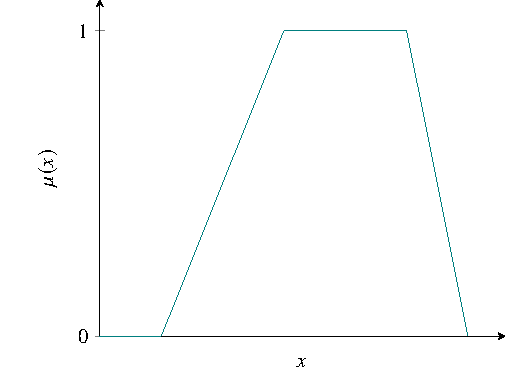
\includegraphics[width=\textwidth]{mf-trapezoid}
        \caption{Trapezoidal MF}
    \end{subfigure}
    %
    \begin{subfigure}[b]{0.4\textwidth}
        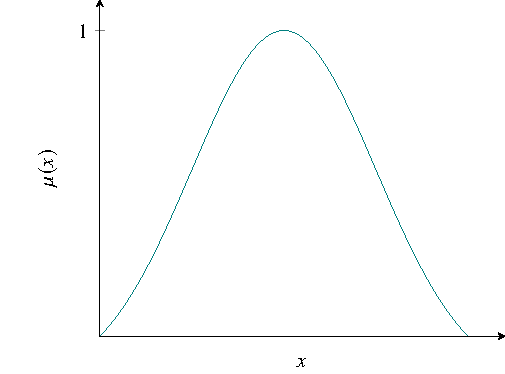
\includegraphics[width=\textwidth]{mf-gauss}
        \caption{Gaussian MF}
    \end{subfigure}
    \begin{subfigure}[b]{0.4\textwidth}
        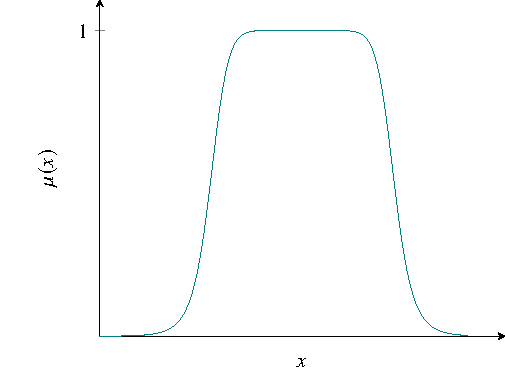
\includegraphics[width=\textwidth]{mf-bell}
        \caption{Generalized bell MF}
    \end{subfigure}
    \begin{subfigure}[b]{0.4\textwidth}
        \vspace{.5em}
        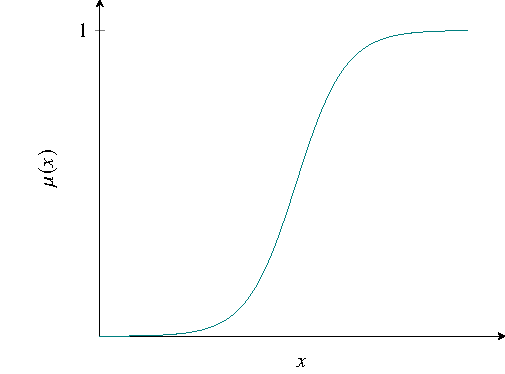
\includegraphics[width=\textwidth]{mf-sigmoid}
        \caption{Sigmoidal MF}
    \end{subfigure}
    \caption{Examples from different membership functions.}
    \label{fig:mfs}
\end{figure}

%--------------------------------------
%  Two-dimensional MFs
%--------------------------------------

\subsection{Two-dimensional MFs}

While it is possible to define membership functions in two or more dimensions, it is often desirable to begin in one dimension and build from there, effectively \textit{extending} the one-dimensional MFs defined above (or any other).

\begin{definition}[Cylindrical extension] If $A$ is a fuzzy set in $X$ and $Y$ is another universe, then the cylindrical extension of $A$ in $X \times Y$ is defined by
\[
c(A) = \int_{X\times Y} \mu_A(x) \slash (x,y).
\]

\end{definition}

We can also perform the inverse operation, that is, decompose a two-dimensional MF in two one-dimensional MFs.

\begin{definition}[Projections] Let $R$ be a two-dimensional fuzzy set on $X\times Y$. Then the projections of $R$ onto $X$ and $Y$ are defined as
\[
R_X = \int_X \max_y \, \mu_R(x,y) \slash x, \quad R_Y = \int_Y \max_x \, \mu_R(x,y) \slash y.
\]

\end{definition}

\begin{definition}[Composite MF] A two-dimensional MF is said to be \textit{composite} if it can be decomposed as an analytic expression of two MFs of one dimension; otherwise it is \textit{non-composite}.

\end{definition}

The Gaussian MF is arguably the most notable example of a composite MF, since it is a well known result that every $n$-dimensional Gaussian function is the product of $n$ one-dimensional Gaussian functions, scaled by some constant factor.


%----------------------------------------
%  Fuzzy Complemnt, T-norm and T-conorm
%----------------------------------------

\subsection{Fuzzy complement, T-norm and T-conorm} \label{ssec:tnorm}

Lastly, we explore the generalization of the classical fuzzy operators that have been described throughout this section.

\begin{definition}[Complement operator] A fuzzy complement operator is a continuous function $N:[0,1] \to [0,1]$ which meets the following axiomatic requirements:

\begin{enumerate}
	\item \textit{(Boundary)} \ $N(0)=1$ and $N(1)=0$;
	\item \textit{(Monotonicity)} \ $N(a) \ge N(b)$ if $a \le b$;
	\item \textit{(Involution)} \ $N(N(a)) = a$.
\end{enumerate}

\end{definition}

\begin{remark} Sometimes an operator verifying only $(i)$ and $(ii)$ is considered a fuzzy complement operator.

\end{remark}

\begin{example} One can routinely verify that the following two operators are fuzzy complement operators.
\begin{enumerate}
  \item \textit{(Sugeno's complement} \cite{sugeno1993fuzzy}$)$ $\displaystyle N_s(a) = \frac{1-a}{1+sa}$, where $s > -1$;
  \vspace{.25em}
  \item \textit{(Yager's complement} \cite{yager1979measure}$)$ $N_w(a) = (1-a^w)^{1/w}$, where $w>0$.
\end{enumerate}

\end{example}

\begin{definition}[$T$-norm operator] The intersection of two fuzzy sets $A$ and $B$ is specified in general by a function $T:[0,1]\times [0,1] \to [0,1]$, referred to as a $T$-norm operator, which aggregates two membership grades,
\[
\mu_{A \cap B}(x) = T(\mu_A(x), \mu_B(x)),
\]
and verifies several basic properties, namely:
\begin{enumerate}
	\item \textit{(Boundary)} \ $T(0,0) = 0$ and $T(a,1) = a$;
	\item \textit{(Monotonicity)} \ $T(a,b) \le T(c,d)$ if $a \le c$ and $b \le d$;
	\item \textit{(Commutativity)} \ $T(a,b) = T(b,a)$;
	\item \textit{(Associativity)} \ $T(a, T(b,c)) = T(T(a,b),c)$.
\end{enumerate}

\end{definition}

For the sake of completeness, here are four of the most frequently used $T$-norm operators:

\begin{enumerate}
	\item \textit{Minimum:} $T_{min}(a,b) = a \land b$;
	\item \textit{Algebraic product:} $T_{ap}(a,b)=ab$;
	\item \textit{Bounded product:} $T_{bp}(a,b) = 0 \lor (a+b-1)$;
	\item \textit{Drastic product:} $T_{dp}(a,b) = \begin{cases}
	                                      a, & \text{if } b = 1,\\
	                                      b, & \text{if } a = 1,\\
	                                      0, & \text{otherwise}.
                                          \end{cases}$
\end{enumerate}

\begin{definition}[$T$-conorm operator] Similarly, the union of two fuzzy sets $A$ and $B$ is specified in general by a function $S:[0,1]\times [0,1] \to [0,1]$, known as a $T$-conorm operator, which works in the same way as a $T$-norm, except that the boundary condition is now $S(1,1) = 1$ and $S(0,a) = a$.

\end{definition}

Corresponding to the four $T$-norm operators previously defined, we have the following $T$-conorm operators:

\begin{enumerate}
	\item \textit{Maximum:} $S_{max}(a,b) = a \lor b$;
	\item \textit{Algebraic sum:} $S_{as}(a,b)=a + b - ab$;
	\item \textit{Bounded sum:} $S_{bs}(a,b) = 1 \land (a+b)$;
	\item \textit{Drastic sum:} $S_{ds}(a,b) = \begin{cases}
	                                      a, & \text{if } b = 0,\\
	                                      b, & \text{if } a = 0,\\
	                                      1, & \text{otherwise}.
                                          \end{cases}$
\end{enumerate}

\begin{theorem}[Generalized De Morgan's Law] $T$-norms and $T$-conorms are duals which support the generalization of De Morgan's law:
\begin{align*}
	T(a,b) &= N(S(N(a),N(b))),\\
	S(a,b) &= N(T(N(a), N(b))).
\end{align*}

\end{theorem}

In fact, the eight operators showed above are dual in the sense of the generalized De Morgan's law.

\section{Fuzzy logic}

In this section we will study the methods and principles of \textit{fuzzy reasoning}, and present fuzzy logic as a multi-valued logic that generalizes the classical two-valued logic. If we think of the predicates \textit{true} and \textit{false} as being codified as $0$ and $1$, respectively, we can understand how to derive a \textit{fuzzy} logic theory in which every predicate has a \textit{truth grade} quantified by an appropiate membership function.

The whole new range of possible truth values gives something of a gray area in which propositions can fall. This is specially interesting in situations which involve a high degree of uncertainty, and thus its structure is difficult to capture with crisp values (if possible at all). The first example that comes to mind is what is known as \textit{natural language processing}, or the modelling of human speech to be ultimately processed by a computer. It is precisely this example that inspires the definitions and concepts that will be presented next, and it can be viewed as the starting point of the subsequent theory.


%--------------------------------------
%  Linguistic Variables
%--------------------------------------

\subsection{Linguistic variables}

\begin{definition}[Linguistic Variable] A linguistic variable is a quintuple $(x, T(x), X, G, M)$, in which

\begin{enumerate}
	\item The symbol $x$ represents the name of the variable;
	\item $T(x)$ is the \textit{term set} of $x$, that is, the set of its \textit{linguistic values};
	\item $X$ is, as usual, the universe of discourse;
	\item $G$ is a \textit{syntactic rule} which generates the terms in $T(x)$;
	\item $M$ is a semantic rule which associates with each linguistic value $A$ its \textit{meaning} $M(A)$, which in turn is nothing more than a fuzzy set in $X$.
\end{enumerate}

\end{definition}

\begin{example}
To help clarify the preceding definition, consider the concept of \textit{age} interpreted as a linguistic variable. Then its term set $T(\text{\textit{age}})$ could be something like the following:
\begin{center}
$T(\text{\textit{age}}) = \left\{\rule{0cm}{1.3cm}\right.$\begin{tabular}{ll}
\textit{young, not young, very young, not very young,} $\dots$, \\
\textit{middle aged, not middle aged,} $\dots$, \\
\textit{old, not old, very old, more or less old, not very old,} $\dots$, \\
\textit{not very young and not very old,}$\dots$
\end{tabular}$\left.\rule{0cm}{1.3cm}\right\}$,
\end{center}
where each term in $T(\text{\textit{age}})$ is characterized by a fuzzy set in a universe $X=[0,100]$.
\end{example}

The syntactic rule refers to the way that linguistic values are generated. We can see that the term set of the previous example consists of several \textit{primary terms} (\textit{young, middle aged, old}) modified by the \textit{negation} (\textit{not}) and/or \textit{adverbs} (\textit{very, more or less, quite,} and so forth), and linked by \textit{connectives} such as \textit{and, or, either} and \textit{neither}.

We shall come up with a way of treating all these modifiers as operators that change the meaning of their operands in a specified, context-independent fashion.

\begin{definition}[Concentration and dilation] Let $A$ be a linguistic value characterized by a fuzzy set with membership function $\mu_A$. Then $A^k$ is interpreted as a modified version of the original linguistic value expressed as
\[
A^k = \int_X (\mu_A(x))^k \slash x.
\]
In particular, the operation of \textit{concentration} is defined as $\operatorname{CON}(A)=A^2$, while that of \textit{dilation} is expressed by $\operatorname{DIL}(A)=A^{0.5}$.

\end{definition}

Conventionally, we take $\operatorname{CON}(A)$ and $\operatorname{DIL}(A)$ to be the result of applying the modifiers \textit{very} and \textit{more or less}, respectively, to the linguistic term $A$. Following the definitions in the previous chapter, we can interpret the negation operator \textit{not} and the connectives \textit{and}, \textit{or} as follows:
\begin{align*}
	\operatorname{NOT}(A) &= \neg A = \int_X 1 - \mu_A(x) \slash x,\\
	A \operatorname{AND} B &= A \cap B = \int_X \mu_A(x) \land \mu_B(x) \slash x,\\
	A \operatorname{OR} B &= A \cup B = \int_X \mu_A(x) \lor \mu_B(x) \slash x.
\end{align*}

\begin{definition}[Contrast intensification] The operation of contrast intensification on a linguistic value $A$ is defined by
\[
\operatorname{INT}(A) = \left\{ \begin{array}{ll}
	2A^2, & \text{if }  0 \le \mu_A(x) \le 0.5,\\
	\neg 2(\neg A)^2, & \text{if }  0.5 \le \mu_A(x) \le 1.
\end{array}\right.
\]
This operator has the effect of reducing the fuzziness of a linguistic value. In the extreme case of repeated applications, the fuzzy set becomes a crisp set with boundaries at the crossover points.

\end{definition}

Lastly, when we define MFs of linguistic values in a term set, it is intuitively reasonable to have these MFs roughly satisfy the requirement of orthogonality, which is described next.

\begin{definition}[Orthogonality] A term set $T= \{t_1, \dots, t_n\}$ of a linguistic variable $x$ on the universe $X$ is \textit{orthogonal} if it fulfills the following property:
\[
\sum_{i=1}^n \mu_{t_i}(x) = 1, \quad \forall x \in X,
\]
where each $t_i$ is a convex and normal fuzzy set defined on $X$.
\end{definition}


%--------------------------------------
%  Fuzzy If-Then Rules
%--------------------------------------

\subsection{Fuzzy if-then rules}

The core idea behind fuzzy reasoning is that the classical if-then rules of inference used in many systems can be reinterpreted under a fuzzy perspective, taking advantage of all the properties and easiness of interpretation that come with it.

\begin{definition}[Fuzzy if-then rules] If $A$ and $B$ are linguistic values, a fuzzy if-then rule associated with them assumes the form
\begin{center}
  if $x$ is $A$ then $y$ is $B$,
\end{center}
where ``$x$ is $A$'' is the \textit{antecedent} part and ``$y$ is $B$'' is the \textit{consequent} part. Sometimes we will abbreviate such a rule as $A\to B$.
\end{definition}

Some examples of fuzzy rules include \textit{if the patient's temperature is high, give them a moderate dose of medicine}, or \textit{tall people will get a big discount}. These rules are most useful, as we have already pointed out, when the concepts we are trying to model are difficult to describe in exact terms: is there a universally accepted height from which a person is considered to be tall? Is a body temperature of 38\textdegree{} indicative of a problem but $37.9$\textdegree{} is not?

Since a fuzzy if-then rule models a relation between two variables $x$ and $y$, it makes sense to interpret $A\to B$ as a fuzzy relation $\mathcal R$ given by a membership function $\mu_{\mathcal R} = f(\mu_A(x), \mu_B(y))$, for an appropiate choice of an implication function $f$ (usually a $T$-norm operator). Now we derive the basic operation of fuzzy reasoning, which consists of an \textit{approximate modus ponens}. Starting from the fuzzy rule \textit{if $x$ is $A$ then $y$ is $B$}, if we have the premise $x$ is $A'$, where $A'$ means an approximation of $A$, we can conclude that $y$ is $B'$, with $B'$ being an approximation of $B$. In other words, if $x$ is $A$ \textit{to a certain degree}, then $y$ is $B$ \textit{to a certain (possibly different) degree}. We give a precise meaning and structure to this process in the following definition.

\begin{definition}[Fuzzy reasoning] Let $X,Y$ be two universes of discourse and let $A, A'$ and $B$ be fuzzy sets in $X$, $X$ and $Y$, respectively. If $A\to B$ is a fuzzy implication, then a fuzzy set $B'$ is induced on $Y$, defined by
\[
B' = A' \circ (A \to B),
\]
where $\circ$ is the max-min composition (see Definition \ref{def:maxmin}), or equivalently,
\[
\mu_{B'}(y) = \lor_x (\mu_{A'}(x) \ \land \mu_{A \to B}(x, y)).
\]

\end{definition}

It goes without saying that we can have as many fuzzy rules as we want, and our ultimate goal will be to aggregate all of them together and produce a coherent reasoning system. Even though we have only considered the simplest case with one antecedent and one consequent, we can treat rules with multiple antecedents using the cartesian product operator, and rules with multiple consequent as the union of many rules with just one consequent. For example, we can have the following line of reasoning:

	\begin{center}
	  $x$ is $A'$ and $t$ is $B'$\\
    if $x$ is $A_1$ and $t$ is $B_1$ then $z$ is $C_1$\\
    if $x$ is $A_2$ and $t$ is $B_2$ then $z$ is $C_2$\\
    \rule{7cm}{0.4pt}\\
    $z$ is $C'$
  \end{center}
In this case, we interpret the first rule as a relation $\mathcal R_1 = A_1 \times B_1 \to C_1$ and the second one as $\mathcal R_2 = A_2 \times B_2 \to C_2$. Then, the induced fuzzy set $C'$ is given by
\[
C' = (A' \times B') \circ (\mathcal R_1 \circ \mathcal R_2) = C_1' \cup C_2',
\]
where $C_1'$ and $C_2'$ are the fuzzy sets inferred from the first and second rule, respectively.

\section{Fuzzy inference systems}

Now that we have gone over all the key elements in the theory of fuzzy reasoning, we are prepared to understand what a \textit{fuzzy inference system} (\acrshort{fis}) is. In summary, it is a system that maps an input space to an output space, using fuzzy techniques along the way as the main reasoning mechanism. Generally speaking it is made of four clearly differentiated parts:

\begin{enumerate}[1.]
  \item A \textit{fuzzification module}, which converts crisp inputs into fuzzy sets, with some predefined membership functions.
  \item A \textit{rulebase} that contains a set of fuzzy if-then rules.
  \item An \textit{inference engine} that takes some input and employs the rules in the rulebase to infer the corresponding output, using the fuzzy reasoning scheme described in the previous section. The membership functions in the output space are also predefined.
  \item A \textit{defuzzifying method} used to convert the output back to a crisp value, if necessary.
\end{enumerate}

A positive quality of a FIS is that its rulebase can be easily modified with the addition of new rules or the adjustment of existing ones. The rules in the rulebase can be defined by an expert based on their knowledge of the specific problem we are tackling, but \textbf{they can also be learned from data}. This fact opens the door to the treatment of fuzzy systems with the techniques and learning algorithms that have been emerging over the course of the last decades in this field. This is precisely what we pursue: to build a fuzzy system that can learn and benefit from enormous amounts of data. This process will be discussed in depth in Chapter \ref{ch:fuzzy-bigdata}.

One of the most important thing to take into account is that the choice of membership function is subjective, but not arbitrary. It heavily depends on the problem we are trying to solve, and selecting the appropiate MF for a given task usually gives much better results than choosing one either at random or one that gave good results on some entirely different problem.

Even though we have described every step of the inferring process in this and the previous sections, we summarize them below for completeness.

\begin{enumerate}[1.]
  \item In the first place, inputs to the system are \textit{fuzzified} and the membership grade of each input to the predefined fuzzy sets are calculated.
  \item Then, the \textit{firing strength} of each rule is computed, which usually consists on performing the fuzzy AND operation between the antecedents.
  \item Now the firing strength of each rule is combined with the consequent part to form an overall degree of satisfaction of the rule, known as the \textit{qualified consequent}. This is done as we described when we talked about implication operators, which in turn are commonly implemented with $T$-norm operators (e.g. the $\land$ operator).
  \item We aggregate all qualified consequents and choose the one that best represents the input value, for which the OR operator is the standard choice.
  \item Finally, we employ the aggregated output MF to obtain a crisp value as the output, i.e. a defuzzified value.
\end{enumerate}

\subsection{Fuzzy system types}

To bring this exposition about fuzzy theory to an end, we present the two most common types of fuzzy systems used in practical applications. These two systems differ mainly in how they treat the output values.

\begin{definition}[Madmani fuzzy inference system] A Madmani fuzzy inference system (see \cite{madmani1975experiment}) is a FIS that takes an input $X=(X_1,\dots,X_n)$ and produces an output $Y = D(Y_1, \dots, Y_m)$, using rules of the form
\begin{center}
  if $X_1$ is $A_1$ and $X_2$ is $A_2$ and $\dots$ and $X_n$ is $A_n$\\
  then $Y_1$ is $B_1$ and $Y_2$ is $B_2$ and $\dots$ and $Y_m$ is $B_m$,
\end{center}
together with a defuzzification function $D:[0,1]^m \to \R^m$ to compute the final crisp values.
\end{definition}

The most common defuzzification method is the \textit{centroid of area} method, or \acrshort{coa} for short. It extracts a representative value from a fuzzy set, which can be thought of as the center of gravity of the area under its membership function. For a one-dimensional fuzzy set $A$ in a universe $Z$, it assumes the form
\[
z = \frac{\int_Z z\mu_A(z)\, dz}{\int_Z \mu_A(z)\, dz}.
\]
Other defuzzification methods are studied in the literature. A non-exhaustive classification of such methods can be found in \cite{leekwijck1999defuzzification}.

\begin{example}
  A typical single-input single-output Madmani fuzzy model could be expressed as follows:
  \[
  \left\{ \begin{array}{l}
	\text{If $X$ is small then $Y$ is small}.\\
  \text{If $X$ is medium then $Y$ is large}.\\
	\text{If $X$ is large then $Y$ is very large}.
\end{array}\right.
\]
\end{example}

The other type of FIS that we will study is one in which the output is not a fuzzy set, but a crisp function of the input values. It is aimed at generating fuzzy rules from a given input-output data set, and is appropiate for solving regression problems.

\begin{definition}[TSK fuzzy inference system] A TSK fuzzy inference system (proposed by Takagi, Sugeno and Kang \cite{takagi1985identification, sugeno1988structure}) is a FIS that takes an input $X=(X_1,\dots,X_n)$ and produces an output $Y = (Y_1, \dots, Y_m)$, using rules of the form
\begin{center}
  if $X_1$ is $A_1$ and $X_2$ is $A_2$ and $\dots$ and $X_n$ is $A_n$\\
  then $Y_1$ is $f_1(X_1, \dots, X_n)$ and $Y_2$ is $f_2(X_1, \dots, X_n)$ and $\dots$ and $Y_m$ is $f_m(X_1, \dots, X_n)$,
\end{center}
where each $f_i$ is a crisp function of the input values (usually a polynomial).
\end{definition}

One thing to take into account is that the overall output is obtained via a \textit{weighted average} of the output of each rule (the weights being their firing strength), since now there are no fuzzy sets in the consequent part. This also eliminates the need for a defuzzification module, and thus improves the speed of the system.

\begin{example}
  A typical single-input TSK fuzzy model could be expressed as follows:
  \[
  \left\{ \begin{array}{l}
	\text{If $X$ is small then $Y=0.1X + 6$}.\\
  \text{If $X$ is medium then $Y=-0.5X -3$}.\\
	\text{If $X$ is large then $Y=X+2$}.
\end{array}\right.
\]
\end{example}
